% Created by tikzDevice version 0.10.1 on 2017-12-13 15:58:48
% !TEX encoding = UTF-8 Unicode
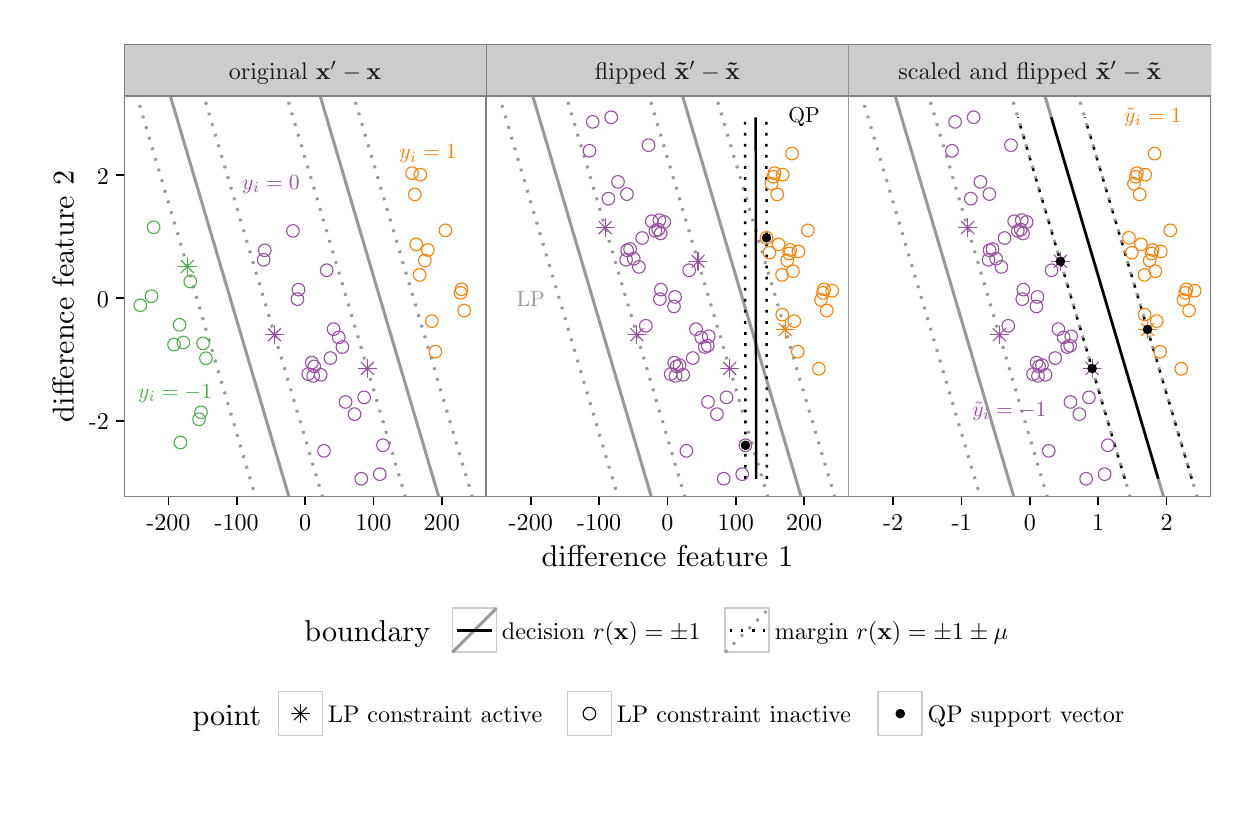
\begin{tikzpicture}[x=1pt,y=1pt]
\definecolor{fillColor}{RGB}{255,255,255}
\path[use as bounding box,fill=fillColor,fill opacity=0.00] (0,0) rectangle (433.62,274.63);
\begin{scope}
\path[clip] (  0.00,  0.00) rectangle (433.62,274.63);
\definecolor{drawColor}{RGB}{255,255,255}
\definecolor{fillColor}{RGB}{255,255,255}

\path[draw=drawColor,line width= 0.6pt,line join=round,line cap=round,fill=fillColor] (  0.00,  0.00) rectangle (433.62,274.63);
\end{scope}
\begin{scope}
\path[clip] ( 34.75,250.04) rectangle (165.70,268.63);
\definecolor{drawColor}{gray}{0.50}
\definecolor{fillColor}{gray}{0.80}

\path[draw=drawColor,line width= 0.2pt,line join=round,line cap=round,fill=fillColor] ( 34.75,250.04) rectangle (165.70,268.63);
\definecolor{drawColor}{gray}{0.10}

\node[text=drawColor,anchor=base,inner sep=0pt, outer sep=0pt, scale=  0.87] at (100.23,256.04) {original $\mathbf x'-\mathbf x$};
\end{scope}
\begin{scope}
\path[clip] (165.70,250.04) rectangle (296.66,268.63);
\definecolor{drawColor}{gray}{0.50}
\definecolor{fillColor}{gray}{0.80}

\path[draw=drawColor,line width= 0.2pt,line join=round,line cap=round,fill=fillColor] (165.70,250.04) rectangle (296.66,268.63);
\definecolor{drawColor}{gray}{0.10}

\node[text=drawColor,anchor=base,inner sep=0pt, outer sep=0pt, scale=  0.87] at (231.18,256.04) {flipped $\mathbf{\tilde x'}-\mathbf{\tilde x}$};
\end{scope}
\begin{scope}
\path[clip] (296.66,250.04) rectangle (427.62,268.63);
\definecolor{drawColor}{gray}{0.50}
\definecolor{fillColor}{gray}{0.80}

\path[draw=drawColor,line width= 0.2pt,line join=round,line cap=round,fill=fillColor] (296.66,250.04) rectangle (427.62,268.63);
\definecolor{drawColor}{gray}{0.10}

\node[text=drawColor,anchor=base,inner sep=0pt, outer sep=0pt, scale=  0.87] at (362.14,256.04) {scaled and flipped $\mathbf{\tilde x'}-\mathbf{\tilde x}$};
\end{scope}
\begin{scope}
\path[clip] ( 34.75,105.04) rectangle (165.70,250.04);
\definecolor{fillColor}{RGB}{255,255,255}

\path[fill=fillColor] ( 34.75,105.04) rectangle (165.70,250.04);
\definecolor{drawColor}{gray}{0.60}

\path[draw=drawColor,line width= 1.1pt,line join=round] ( 44.25,274.63) -- (125.52,  0.00);

\path[draw=drawColor,line width= 1.1pt,line join=round] ( 98.39,274.63) -- (165.70, 47.12);

\path[draw=drawColor,line width= 1.1pt,dash pattern=on 1pt off 3pt ,line join=round] ( 86.29,274.63) -- (165.70,  6.24);

\path[draw=drawColor,line width= 1.1pt,dash pattern=on 1pt off 3pt ,line join=round] (110.48,274.63) -- (165.70, 88.01);

\path[draw=drawColor,line width= 1.1pt,dash pattern=on 1pt off 3pt ,line join=round] ( 34.75,265.87) -- (113.42,  0.00);

\path[draw=drawColor,line width= 1.1pt,dash pattern=on 1pt off 3pt ,line join=round] ( 56.35,274.63) -- (137.62,  0.00);
\definecolor{drawColor}{RGB}{152,78,163}

\path[draw=drawColor,line width= 0.4pt,line join=round,line cap=round] (105.90,149.19) circle (  2.28);

\path[draw=drawColor,line width= 0.4pt,line join=round,line cap=round] (118.10,134.98) circle (  2.28);

\path[draw=drawColor,line width= 0.4pt,line join=round,line cap=round] (120.55,111.63) circle (  2.28);

\path[draw=drawColor,line width= 0.4pt,line join=round,line cap=round] (128.40,123.74) circle (  2.28);

\path[draw=drawColor,line width= 0.4pt,line join=round,line cap=round] (103.16,148.80) circle (  2.28);

\path[draw=drawColor,line width= 0.4pt,line join=round,line cap=round] (127.24,113.29) circle (  2.28);

\path[draw=drawColor,line width= 0.4pt,line join=round,line cap=round] (113.73,159.23) circle (  2.28);

\path[draw=drawColor,line width= 0.4pt,line join=round,line cap=round] (103.54,152.23) circle (  2.28);

\path[draw=drawColor,line width= 0.4pt,line join=round,line cap=round] (107.06,121.71) circle (  2.28);
\definecolor{drawColor}{RGB}{255,127,0}

\path[draw=drawColor,line width= 0.4pt,line join=round,line cap=round] (139.89,214.37) circle (  2.28);

\path[draw=drawColor,line width= 0.4pt,line join=round,line cap=round] (141.88,221.51) circle (  2.28);
\definecolor{drawColor}{RGB}{77,175,74}

\path[draw=drawColor,line width= 0.4pt,line join=round,line cap=round] ( 62.62,135.64) circle (  2.28);

\path[draw=drawColor,line width= 0.4pt,line join=round,line cap=round] ( 63.38,160.55) circle (  2.28);

\path[draw=drawColor,line width= 0.4pt,line join=round,line cap=round] ( 61.92,133.12) circle (  2.28);
\definecolor{drawColor}{RGB}{255,127,0}

\path[draw=drawColor,line width= 0.4pt,line join=round,line cap=round] (138.91,222.04) circle (  2.28);

\path[draw=drawColor,line width= 0.4pt,line join=round,line cap=round] (141.64,185.30) circle (  2.28);
\definecolor{drawColor}{RGB}{77,175,74}

\path[draw=drawColor,line width= 0.4pt,line join=round,line cap=round] ( 64.43,155.18) circle (  2.28);

\path[draw=drawColor,line width= 0.4pt,line join=round,line cap=round] ( 55.18,124.74) circle (  2.28);
\definecolor{drawColor}{RGB}{255,127,0}

\path[draw=drawColor,line width= 0.4pt,line join=round,line cap=round] (140.38,196.34) circle (  2.28);
\definecolor{drawColor}{RGB}{152,78,163}

\path[draw=drawColor,line width= 0.4pt,line join=round,line cap=round] (112.42,162.72) circle (  2.28);

\path[draw=drawColor,line width= 0.4pt,line join=round,line cap=round] (114.87,139.38) circle (  2.28);

\path[draw=drawColor,line width= 0.4pt,line join=round,line cap=round] (120.44,149.20) -- (125.01,153.77);

\path[draw=drawColor,line width= 0.4pt,line join=round,line cap=round] (120.44,153.77) -- (125.01,149.20);

\path[draw=drawColor,line width= 0.4pt,line join=round,line cap=round] (119.50,151.49) -- (125.95,151.49);

\path[draw=drawColor,line width= 0.4pt,line join=round,line cap=round] (122.72,148.26) -- (122.72,154.72);

\path[draw=drawColor,line width= 0.4pt,line join=round,line cap=round] ( 97.48,176.55) circle (  2.28);

\path[draw=drawColor,line width= 0.4pt,line join=round,line cap=round] (121.57,141.04) circle (  2.28);

\path[draw=drawColor,line width= 0.4pt,line join=round,line cap=round] (108.05,186.98) circle (  2.28);

\path[draw=drawColor,line width= 0.4pt,line join=round,line cap=round] ( 97.86,179.97) circle (  2.28);

\path[draw=drawColor,line width= 0.4pt,line join=round,line cap=round] (101.38,149.45) circle (  2.28);
\definecolor{drawColor}{RGB}{77,175,74}

\path[draw=drawColor,line width= 0.4pt,line join=round,line cap=round] ( 54.88,167.25) circle (  2.28);

\path[draw=drawColor,line width= 0.4pt,line join=round,line cap=round] ( 52.90,160.11) circle (  2.28);
\definecolor{drawColor}{RGB}{255,127,0}

\path[draw=drawColor,line width= 0.4pt,line join=round,line cap=round] (143.51,190.49) circle (  2.28);
\definecolor{drawColor}{RGB}{77,175,74}

\path[draw=drawColor,line width= 0.4pt,line join=round,line cap=round] ( 55.42,186.01) -- ( 59.98,190.58);

\path[draw=drawColor,line width= 0.4pt,line join=round,line cap=round] ( 55.42,190.58) -- ( 59.98,186.01);

\path[draw=drawColor,line width= 0.4pt,line join=round,line cap=round] ( 54.47,188.30) -- ( 60.93,188.30);

\path[draw=drawColor,line width= 0.4pt,line join=round,line cap=round] ( 57.70,185.07) -- ( 57.70,191.52);

\path[draw=drawColor,line width= 0.4pt,line join=round,line cap=round] ( 56.25,160.87) circle (  2.28);
\definecolor{drawColor}{RGB}{255,127,0}

\path[draw=drawColor,line width= 0.4pt,line join=round,line cap=round] (144.59,194.30) circle (  2.28);

\path[draw=drawColor,line width= 0.4pt,line join=round,line cap=round] (147.32,157.55) circle (  2.28);
\definecolor{drawColor}{RGB}{77,175,74}

\path[draw=drawColor,line width= 0.4pt,line join=round,line cap=round] ( 58.75,182.93) circle (  2.28);
\definecolor{drawColor}{RGB}{255,127,0}

\path[draw=drawColor,line width= 0.4pt,line join=round,line cap=round] (150.95,201.39) circle (  2.28);

\path[draw=drawColor,line width= 0.4pt,line join=round,line cap=round] (146.06,168.59) circle (  2.28);
\definecolor{drawColor}{RGB}{152,78,163}

\path[draw=drawColor,line width= 0.4pt,line join=round,line cap=round] (102.68,153.59) circle (  2.28);

\path[draw=drawColor,line width= 0.4pt,line join=round,line cap=round] (110.53,165.70) circle (  2.28);

\path[draw=drawColor,line width= 0.4pt,line join=round,line cap=round] ( 85.28,190.76) circle (  2.28);

\path[draw=drawColor,line width= 0.4pt,line join=round,line cap=round] (109.37,155.25) circle (  2.28);

\path[draw=drawColor,line width= 0.4pt,line join=round,line cap=round] ( 95.85,201.19) circle (  2.28);

\path[draw=drawColor,line width= 0.4pt,line join=round,line cap=round] ( 85.67,194.19) circle (  2.28);

\path[draw=drawColor,line width= 0.4pt,line join=round,line cap=round] ( 86.90,161.38) -- ( 91.47,165.95);

\path[draw=drawColor,line width= 0.4pt,line join=round,line cap=round] ( 86.90,165.95) -- ( 91.47,161.38);

\path[draw=drawColor,line width= 0.4pt,line join=round,line cap=round] ( 85.96,163.67) -- ( 92.41,163.67);

\path[draw=drawColor,line width= 0.4pt,line join=round,line cap=round] ( 89.18,160.44) -- ( 89.18,166.90);
\definecolor{drawColor}{RGB}{255,127,0}

\path[draw=drawColor,line width= 0.4pt,line join=round,line cap=round] (157.76,172.41) circle (  2.28);
\definecolor{drawColor}{RGB}{77,175,74}

\path[draw=drawColor,line width= 0.4pt,line join=round,line cap=round] ( 40.70,174.33) circle (  2.28);

\path[draw=drawColor,line width= 0.4pt,line join=round,line cap=round] ( 44.75,177.60) circle (  2.28);

\path[draw=drawColor,line width= 0.4pt,line join=round,line cap=round] ( 45.50,202.51) circle (  2.28);
\definecolor{drawColor}{RGB}{255,127,0}

\path[draw=drawColor,line width= 0.4pt,line join=round,line cap=round] (156.40,178.79) circle (  2.28);

\path[draw=drawColor,line width= 0.4pt,line join=round,line cap=round] (156.78,180.08) circle (  2.28);
\definecolor{drawColor}{RGB}{77,175,74}

\node[text=drawColor,anchor=base,inner sep=0pt, outer sep=0pt, scale=  0.78] at ( 53.30,140.75) {$y_i=-1$};
\definecolor{drawColor}{RGB}{152,78,163}

\node[text=drawColor,anchor=base,inner sep=0pt, outer sep=0pt, scale=  0.78] at ( 87.88,216.14) {$y_i=0$};
\definecolor{drawColor}{RGB}{255,127,0}

\node[text=drawColor,anchor=base,inner sep=0pt, outer sep=0pt, scale=  0.78] at (144.68,227.22) {$y_i=1$};
\definecolor{drawColor}{gray}{0.50}

\path[draw=drawColor,line width= 0.6pt,line join=round,line cap=round] ( 34.75,105.04) rectangle (165.70,250.04);
\end{scope}
\begin{scope}
\path[clip] (165.70,105.04) rectangle (296.66,250.04);
\definecolor{fillColor}{RGB}{255,255,255}

\path[fill=fillColor] (165.70,105.04) rectangle (296.66,250.04);
\definecolor{drawColor}{gray}{0.60}

\path[draw=drawColor,line width= 1.1pt,line join=round] (175.21,274.63) -- (256.47,  0.00);

\path[draw=drawColor,line width= 1.1pt,line join=round] (229.34,274.63) -- (296.66, 47.12);

\path[draw=drawColor,line width= 1.1pt,dash pattern=on 1pt off 3pt ,line join=round] (217.24,274.63) -- (296.66,  6.24);

\path[draw=drawColor,line width= 1.1pt,dash pattern=on 1pt off 3pt ,line join=round] (241.44,274.63) -- (296.66, 88.01);

\path[draw=drawColor,line width= 1.1pt,dash pattern=on 1pt off 3pt ,line join=round] (165.70,265.87) -- (244.38,  0.00);

\path[draw=drawColor,line width= 1.1pt,dash pattern=on 1pt off 3pt ,line join=round] (187.31,274.63) -- (268.57,  0.00);
\definecolor{drawColor}{RGB}{0,0,0}

\path[draw=drawColor,line width= 0.9pt,dash pattern=on 1pt off 3pt ,line join=round] (259.36,111.63) -- (259.20,242.24);

\path[draw=drawColor,line width= 0.9pt,dash pattern=on 1pt off 3pt ,line join=round] (267.10,111.63) -- (266.94,242.24);

\path[draw=drawColor,line width= 0.9pt,line join=round] (263.23,111.63) -- (263.07,242.24);

\node[text=drawColor,anchor=base,inner sep=0pt, outer sep=0pt, scale=  0.78] at (280.58,240.53) {QP};
\definecolor{drawColor}{gray}{0.60}

\node[text=drawColor,anchor=base,inner sep=0pt, outer sep=0pt, scale=  0.78] at (181.79,174.01) {LP};
\definecolor{drawColor}{RGB}{152,78,163}

\path[draw=drawColor,line width= 0.4pt,line join=round,line cap=round] (236.86,149.19) circle (  2.28);

\path[draw=drawColor,line width= 0.4pt,line join=round,line cap=round] (249.06,134.98) circle (  2.28);

\path[draw=drawColor,line width= 0.4pt,line join=round,line cap=round] (251.51,111.63) circle (  2.28);

\path[draw=drawColor,line width= 0.4pt,line join=round,line cap=round] (259.36,123.74) circle (  2.28);

\path[draw=drawColor,line width= 0.4pt,line join=round,line cap=round] (234.12,148.80) circle (  2.28);

\path[draw=drawColor,line width= 0.4pt,line join=round,line cap=round] (258.20,113.29) circle (  2.28);

\path[draw=drawColor,line width= 0.4pt,line join=round,line cap=round] (244.68,159.23) circle (  2.28);

\path[draw=drawColor,line width= 0.4pt,line join=round,line cap=round] (234.50,152.23) circle (  2.28);

\path[draw=drawColor,line width= 0.4pt,line join=round,line cap=round] (238.02,121.71) circle (  2.28);
\definecolor{drawColor}{RGB}{255,127,0}

\path[draw=drawColor,line width= 0.4pt,line join=round,line cap=round] (270.85,214.37) circle (  2.28);

\path[draw=drawColor,line width= 0.4pt,line join=round,line cap=round] (272.84,221.51) circle (  2.28);

\path[draw=drawColor,line width= 0.4pt,line join=round,line cap=round] (268.79,218.24) circle (  2.28);

\path[draw=drawColor,line width= 0.4pt,line join=round,line cap=round] (268.03,193.33) circle (  2.28);

\path[draw=drawColor,line width= 0.4pt,line join=round,line cap=round] (269.48,220.75) circle (  2.28);

\path[draw=drawColor,line width= 0.4pt,line join=round,line cap=round] (269.87,222.04) circle (  2.28);

\path[draw=drawColor,line width= 0.4pt,line join=round,line cap=round] (272.60,185.30) circle (  2.28);

\path[draw=drawColor,line width= 0.4pt,line join=round,line cap=round] (266.98,198.69) circle (  2.28);

\path[draw=drawColor,line width= 0.4pt,line join=round,line cap=round] (276.23,229.13) circle (  2.28);

\path[draw=drawColor,line width= 0.4pt,line join=round,line cap=round] (271.34,196.34) circle (  2.28);
\definecolor{drawColor}{RGB}{152,78,163}

\path[draw=drawColor,line width= 0.4pt,line join=round,line cap=round] (243.38,162.72) circle (  2.28);

\path[draw=drawColor,line width= 0.4pt,line join=round,line cap=round] (245.83,139.38) circle (  2.28);

\path[draw=drawColor,line width= 0.4pt,line join=round,line cap=round] (251.40,149.20) -- (255.97,153.77);

\path[draw=drawColor,line width= 0.4pt,line join=round,line cap=round] (251.40,153.77) -- (255.97,149.20);

\path[draw=drawColor,line width= 0.4pt,line join=round,line cap=round] (250.45,151.49) -- (256.91,151.49);

\path[draw=drawColor,line width= 0.4pt,line join=round,line cap=round] (253.68,148.26) -- (253.68,154.72);

\path[draw=drawColor,line width= 0.4pt,line join=round,line cap=round] (228.44,176.55) circle (  2.28);

\path[draw=drawColor,line width= 0.4pt,line join=round,line cap=round] (252.52,141.04) circle (  2.28);

\path[draw=drawColor,line width= 0.4pt,line join=round,line cap=round] (239.01,186.98) circle (  2.28);

\path[draw=drawColor,line width= 0.4pt,line join=round,line cap=round] (228.82,179.97) circle (  2.28);

\path[draw=drawColor,line width= 0.4pt,line join=round,line cap=round] (232.34,149.45) circle (  2.28);
\definecolor{drawColor}{RGB}{255,127,0}

\path[draw=drawColor,line width= 0.4pt,line join=round,line cap=round] (276.53,186.63) circle (  2.28);

\path[draw=drawColor,line width= 0.4pt,line join=round,line cap=round] (278.51,193.76) circle (  2.28);

\path[draw=drawColor,line width= 0.4pt,line join=round,line cap=round] (274.46,190.49) circle (  2.28);

\path[draw=drawColor,line width= 0.4pt,line join=round,line cap=round] (271.42,163.30) -- (275.99,167.86);

\path[draw=drawColor,line width= 0.4pt,line join=round,line cap=round] (271.42,167.86) -- (275.99,163.30);

\path[draw=drawColor,line width= 0.4pt,line join=round,line cap=round] (270.48,165.58) -- (276.94,165.58);

\path[draw=drawColor,line width= 0.4pt,line join=round,line cap=round] (273.71,162.35) -- (273.71,168.81);

\path[draw=drawColor,line width= 0.4pt,line join=round,line cap=round] (275.16,193.01) circle (  2.28);

\path[draw=drawColor,line width= 0.4pt,line join=round,line cap=round] (275.54,194.30) circle (  2.28);

\path[draw=drawColor,line width= 0.4pt,line join=round,line cap=round] (278.28,157.55) circle (  2.28);

\path[draw=drawColor,line width= 0.4pt,line join=round,line cap=round] (272.66,170.95) circle (  2.28);

\path[draw=drawColor,line width= 0.4pt,line join=round,line cap=round] (281.91,201.39) circle (  2.28);

\path[draw=drawColor,line width= 0.4pt,line join=round,line cap=round] (277.01,168.59) circle (  2.28);
\definecolor{drawColor}{RGB}{152,78,163}

\path[draw=drawColor,line width= 0.4pt,line join=round,line cap=round] (233.63,153.59) circle (  2.28);

\path[draw=drawColor,line width= 0.4pt,line join=round,line cap=round] (241.49,165.70) circle (  2.28);

\path[draw=drawColor,line width= 0.4pt,line join=round,line cap=round] (216.24,190.76) circle (  2.28);

\path[draw=drawColor,line width= 0.4pt,line join=round,line cap=round] (240.33,155.25) circle (  2.28);

\path[draw=drawColor,line width= 0.4pt,line join=round,line cap=round] (226.81,201.19) circle (  2.28);

\path[draw=drawColor,line width= 0.4pt,line join=round,line cap=round] (216.62,194.19) circle (  2.28);

\path[draw=drawColor,line width= 0.4pt,line join=round,line cap=round] (217.86,161.38) -- (222.43,165.95);

\path[draw=drawColor,line width= 0.4pt,line join=round,line cap=round] (217.86,165.95) -- (222.43,161.38);

\path[draw=drawColor,line width= 0.4pt,line join=round,line cap=round] (216.91,163.67) -- (223.37,163.67);

\path[draw=drawColor,line width= 0.4pt,line join=round,line cap=round] (220.14,160.44) -- (220.14,166.90);
\definecolor{drawColor}{RGB}{255,127,0}

\path[draw=drawColor,line width= 0.4pt,line join=round,line cap=round] (288.72,172.41) circle (  2.28);

\path[draw=drawColor,line width= 0.4pt,line join=round,line cap=round] (290.71,179.55) circle (  2.28);

\path[draw=drawColor,line width= 0.4pt,line join=round,line cap=round] (286.66,176.28) circle (  2.28);

\path[draw=drawColor,line width= 0.4pt,line join=round,line cap=round] (285.90,151.37) circle (  2.28);

\path[draw=drawColor,line width= 0.4pt,line join=round,line cap=round] (287.36,178.79) circle (  2.28);

\path[draw=drawColor,line width= 0.4pt,line join=round,line cap=round] (287.74,180.08) circle (  2.28);
\definecolor{drawColor}{RGB}{152,78,163}

\path[draw=drawColor,line width= 0.4pt,line join=round,line cap=round] (225.51,204.68) circle (  2.28);

\path[draw=drawColor,line width= 0.4pt,line join=round,line cap=round] (213.31,218.90) circle (  2.28);

\path[draw=drawColor,line width= 0.4pt,line join=round,line cap=round] (210.86,242.24) circle (  2.28);

\path[draw=drawColor,line width= 0.4pt,line join=round,line cap=round] (203.01,230.14) circle (  2.28);

\path[draw=drawColor,line width= 0.4pt,line join=round,line cap=round] (228.25,205.07) circle (  2.28);

\path[draw=drawColor,line width= 0.4pt,line join=round,line cap=round] (204.17,240.59) circle (  2.28);

\path[draw=drawColor,line width= 0.4pt,line join=round,line cap=round] (217.68,194.64) circle (  2.28);

\path[draw=drawColor,line width= 0.4pt,line join=round,line cap=round] (227.87,201.65) circle (  2.28);

\path[draw=drawColor,line width= 0.4pt,line join=round,line cap=round] (224.35,232.17) circle (  2.28);

\path[draw=drawColor,line width= 0.4pt,line join=round,line cap=round] (218.99,191.15) circle (  2.28);

\path[draw=drawColor,line width= 0.4pt,line join=round,line cap=round] (216.54,214.50) circle (  2.28);

\path[draw=drawColor,line width= 0.4pt,line join=round,line cap=round] (206.40,200.11) -- (210.97,204.67);

\path[draw=drawColor,line width= 0.4pt,line join=round,line cap=round] (206.40,204.67) -- (210.97,200.11);

\path[draw=drawColor,line width= 0.4pt,line join=round,line cap=round] (205.46,202.39) -- (211.91,202.39);

\path[draw=drawColor,line width= 0.4pt,line join=round,line cap=round] (208.68,199.16) -- (208.68,205.62);

\path[draw=drawColor,line width= 0.4pt,line join=round,line cap=round] (233.93,177.33) circle (  2.28);

\path[draw=drawColor,line width= 0.4pt,line join=round,line cap=round] (209.84,212.84) circle (  2.28);

\path[draw=drawColor,line width= 0.4pt,line join=round,line cap=round] (223.36,166.90) circle (  2.28);

\path[draw=drawColor,line width= 0.4pt,line join=round,line cap=round] (233.55,173.90) circle (  2.28);

\path[draw=drawColor,line width= 0.4pt,line join=round,line cap=round] (230.03,204.42) circle (  2.28);

\path[draw=drawColor,line width= 0.4pt,line join=round,line cap=round] (228.73,200.28) circle (  2.28);

\path[draw=drawColor,line width= 0.4pt,line join=round,line cap=round] (220.88,188.17) circle (  2.28);

\path[draw=drawColor,line width= 0.4pt,line join=round,line cap=round] (246.12,163.11) circle (  2.28);

\path[draw=drawColor,line width= 0.4pt,line join=round,line cap=round] (222.04,198.62) circle (  2.28);

\path[draw=drawColor,line width= 0.4pt,line join=round,line cap=round] (235.56,152.68) circle (  2.28);

\path[draw=drawColor,line width= 0.4pt,line join=round,line cap=round] (245.74,159.69) circle (  2.28);

\path[draw=drawColor,line width= 0.4pt,line join=round,line cap=round] (239.94,187.93) -- (244.51,192.49);

\path[draw=drawColor,line width= 0.4pt,line join=round,line cap=round] (239.94,192.49) -- (244.51,187.93);

\path[draw=drawColor,line width= 0.4pt,line join=round,line cap=round] (239.00,190.21) -- (245.45,190.21);

\path[draw=drawColor,line width= 0.4pt,line join=round,line cap=round] (242.22,186.98) -- (242.22,193.44);
\definecolor{drawColor}{RGB}{0,0,0}
\definecolor{fillColor}{RGB}{0,0,0}

\path[draw=drawColor,line width= 0.4pt,line join=round,line cap=round,fill=fillColor] (259.36,123.74) circle (  1.52);

\path[draw=drawColor,line width= 0.4pt,line join=round,line cap=round,fill=fillColor] (266.98,198.69) circle (  1.52);
\definecolor{drawColor}{gray}{0.50}

\path[draw=drawColor,line width= 0.6pt,line join=round,line cap=round] (165.70,105.04) rectangle (296.66,250.04);
\end{scope}
\begin{scope}
\path[clip] (296.66,105.04) rectangle (427.62,250.04);
\definecolor{fillColor}{RGB}{255,255,255}

\path[fill=fillColor] (296.66,105.04) rectangle (427.62,250.04);
\definecolor{drawColor}{gray}{0.60}

\path[draw=drawColor,line width= 1.1pt,line join=round] (306.17,274.63) -- (387.43,  0.00);

\path[draw=drawColor,line width= 1.1pt,line join=round] (360.30,274.63) -- (427.62, 47.12);

\path[draw=drawColor,line width= 1.1pt,dash pattern=on 1pt off 3pt ,line join=round] (348.20,274.63) -- (427.62,  6.24);

\path[draw=drawColor,line width= 1.1pt,dash pattern=on 1pt off 3pt ,line join=round] (372.40,274.63) -- (427.62, 88.01);

\path[draw=drawColor,line width= 1.1pt,dash pattern=on 1pt off 3pt ,line join=round] (296.66,265.87) -- (375.33,  0.00);

\path[draw=drawColor,line width= 1.1pt,dash pattern=on 1pt off 3pt ,line join=round] (318.27,274.63) -- (399.53,  0.00);
\definecolor{drawColor}{RGB}{0,0,0}

\path[draw=drawColor,line width= 0.9pt,dash pattern=on 1pt off 3pt ,line join=round] (396.43,111.63) -- (357.78,242.24);

\path[draw=drawColor,line width= 0.9pt,dash pattern=on 1pt off 3pt ,line join=round] (420.63,111.63) -- (381.98,242.24);

\path[draw=drawColor,line width= 0.9pt,line join=round] (408.53,111.63) -- (369.88,242.24);
\definecolor{drawColor}{RGB}{152,78,163}

\path[draw=drawColor,line width= 0.4pt,line join=round,line cap=round] (367.82,149.19) circle (  2.28);

\path[draw=drawColor,line width= 0.4pt,line join=round,line cap=round] (380.01,134.98) circle (  2.28);

\path[draw=drawColor,line width= 0.4pt,line join=round,line cap=round] (382.46,111.63) circle (  2.28);

\path[draw=drawColor,line width= 0.4pt,line join=round,line cap=round] (390.32,123.74) circle (  2.28);

\path[draw=drawColor,line width= 0.4pt,line join=round,line cap=round] (365.07,148.80) circle (  2.28);

\path[draw=drawColor,line width= 0.4pt,line join=round,line cap=round] (389.16,113.29) circle (  2.28);

\path[draw=drawColor,line width= 0.4pt,line join=round,line cap=round] (375.64,159.23) circle (  2.28);

\path[draw=drawColor,line width= 0.4pt,line join=round,line cap=round] (365.45,152.23) circle (  2.28);

\path[draw=drawColor,line width= 0.4pt,line join=round,line cap=round] (368.97,121.71) circle (  2.28);
\definecolor{drawColor}{RGB}{255,127,0}

\path[draw=drawColor,line width= 0.4pt,line join=round,line cap=round] (401.81,214.37) circle (  2.28);

\path[draw=drawColor,line width= 0.4pt,line join=round,line cap=round] (403.79,221.51) circle (  2.28);

\path[draw=drawColor,line width= 0.4pt,line join=round,line cap=round] (399.75,218.24) circle (  2.28);

\path[draw=drawColor,line width= 0.4pt,line join=round,line cap=round] (398.99,193.33) circle (  2.28);

\path[draw=drawColor,line width= 0.4pt,line join=round,line cap=round] (400.44,220.75) circle (  2.28);

\path[draw=drawColor,line width= 0.4pt,line join=round,line cap=round] (400.83,222.04) circle (  2.28);

\path[draw=drawColor,line width= 0.4pt,line join=round,line cap=round] (403.56,185.30) circle (  2.28);

\path[draw=drawColor,line width= 0.4pt,line join=round,line cap=round] (397.94,198.69) circle (  2.28);

\path[draw=drawColor,line width= 0.4pt,line join=round,line cap=round] (407.19,229.13) circle (  2.28);

\path[draw=drawColor,line width= 0.4pt,line join=round,line cap=round] (402.29,196.34) circle (  2.28);
\definecolor{drawColor}{RGB}{152,78,163}

\path[draw=drawColor,line width= 0.4pt,line join=round,line cap=round] (374.34,162.72) circle (  2.28);

\path[draw=drawColor,line width= 0.4pt,line join=round,line cap=round] (376.79,139.38) circle (  2.28);

\path[draw=drawColor,line width= 0.4pt,line join=round,line cap=round] (382.36,149.20) -- (386.92,153.77);

\path[draw=drawColor,line width= 0.4pt,line join=round,line cap=round] (382.36,153.77) -- (386.92,149.20);

\path[draw=drawColor,line width= 0.4pt,line join=round,line cap=round] (381.41,151.49) -- (387.87,151.49);

\path[draw=drawColor,line width= 0.4pt,line join=round,line cap=round] (384.64,148.26) -- (384.64,154.72);

\path[draw=drawColor,line width= 0.4pt,line join=round,line cap=round] (359.40,176.55) circle (  2.28);

\path[draw=drawColor,line width= 0.4pt,line join=round,line cap=round] (383.48,141.04) circle (  2.28);

\path[draw=drawColor,line width= 0.4pt,line join=round,line cap=round] (369.97,186.98) circle (  2.28);

\path[draw=drawColor,line width= 0.4pt,line join=round,line cap=round] (359.78,179.97) circle (  2.28);

\path[draw=drawColor,line width= 0.4pt,line join=round,line cap=round] (363.30,149.45) circle (  2.28);
\definecolor{drawColor}{RGB}{255,127,0}

\path[draw=drawColor,line width= 0.4pt,line join=round,line cap=round] (407.48,186.63) circle (  2.28);

\path[draw=drawColor,line width= 0.4pt,line join=round,line cap=round] (409.47,193.76) circle (  2.28);

\path[draw=drawColor,line width= 0.4pt,line join=round,line cap=round] (405.42,190.49) circle (  2.28);

\path[draw=drawColor,line width= 0.4pt,line join=round,line cap=round] (402.38,163.30) -- (406.95,167.86);

\path[draw=drawColor,line width= 0.4pt,line join=round,line cap=round] (402.38,167.86) -- (406.95,163.30);

\path[draw=drawColor,line width= 0.4pt,line join=round,line cap=round] (401.44,165.58) -- (407.89,165.58);

\path[draw=drawColor,line width= 0.4pt,line join=round,line cap=round] (404.67,162.35) -- (404.67,168.81);

\path[draw=drawColor,line width= 0.4pt,line join=round,line cap=round] (406.12,193.01) circle (  2.28);

\path[draw=drawColor,line width= 0.4pt,line join=round,line cap=round] (406.50,194.30) circle (  2.28);

\path[draw=drawColor,line width= 0.4pt,line join=round,line cap=round] (409.23,157.55) circle (  2.28);

\path[draw=drawColor,line width= 0.4pt,line join=round,line cap=round] (403.61,170.95) circle (  2.28);

\path[draw=drawColor,line width= 0.4pt,line join=round,line cap=round] (412.87,201.39) circle (  2.28);

\path[draw=drawColor,line width= 0.4pt,line join=round,line cap=round] (407.97,168.59) circle (  2.28);
\definecolor{drawColor}{RGB}{152,78,163}

\path[draw=drawColor,line width= 0.4pt,line join=round,line cap=round] (364.59,153.59) circle (  2.28);

\path[draw=drawColor,line width= 0.4pt,line join=round,line cap=round] (372.44,165.70) circle (  2.28);

\path[draw=drawColor,line width= 0.4pt,line join=round,line cap=round] (347.20,190.76) circle (  2.28);

\path[draw=drawColor,line width= 0.4pt,line join=round,line cap=round] (371.29,155.25) circle (  2.28);

\path[draw=drawColor,line width= 0.4pt,line join=round,line cap=round] (357.77,201.19) circle (  2.28);

\path[draw=drawColor,line width= 0.4pt,line join=round,line cap=round] (347.58,194.19) circle (  2.28);

\path[draw=drawColor,line width= 0.4pt,line join=round,line cap=round] (348.82,161.38) -- (353.38,165.95);

\path[draw=drawColor,line width= 0.4pt,line join=round,line cap=round] (348.82,165.95) -- (353.38,161.38);

\path[draw=drawColor,line width= 0.4pt,line join=round,line cap=round] (347.87,163.67) -- (354.33,163.67);

\path[draw=drawColor,line width= 0.4pt,line join=round,line cap=round] (351.10,160.44) -- (351.10,166.90);
\definecolor{drawColor}{RGB}{255,127,0}

\path[draw=drawColor,line width= 0.4pt,line join=round,line cap=round] (419.68,172.41) circle (  2.28);

\path[draw=drawColor,line width= 0.4pt,line join=round,line cap=round] (421.67,179.55) circle (  2.28);

\path[draw=drawColor,line width= 0.4pt,line join=round,line cap=round] (417.62,176.28) circle (  2.28);

\path[draw=drawColor,line width= 0.4pt,line join=round,line cap=round] (416.86,151.37) circle (  2.28);

\path[draw=drawColor,line width= 0.4pt,line join=round,line cap=round] (418.31,178.79) circle (  2.28);

\path[draw=drawColor,line width= 0.4pt,line join=round,line cap=round] (418.70,180.08) circle (  2.28);
\definecolor{drawColor}{RGB}{152,78,163}

\path[draw=drawColor,line width= 0.4pt,line join=round,line cap=round] (356.47,204.68) circle (  2.28);

\path[draw=drawColor,line width= 0.4pt,line join=round,line cap=round] (344.27,218.90) circle (  2.28);

\path[draw=drawColor,line width= 0.4pt,line join=round,line cap=round] (341.82,242.24) circle (  2.28);

\path[draw=drawColor,line width= 0.4pt,line join=round,line cap=round] (333.97,230.14) circle (  2.28);

\path[draw=drawColor,line width= 0.4pt,line join=round,line cap=round] (359.21,205.07) circle (  2.28);

\path[draw=drawColor,line width= 0.4pt,line join=round,line cap=round] (335.12,240.59) circle (  2.28);

\path[draw=drawColor,line width= 0.4pt,line join=round,line cap=round] (348.64,194.64) circle (  2.28);

\path[draw=drawColor,line width= 0.4pt,line join=round,line cap=round] (358.83,201.65) circle (  2.28);

\path[draw=drawColor,line width= 0.4pt,line join=round,line cap=round] (355.31,232.17) circle (  2.28);

\path[draw=drawColor,line width= 0.4pt,line join=round,line cap=round] (349.94,191.15) circle (  2.28);

\path[draw=drawColor,line width= 0.4pt,line join=round,line cap=round] (347.50,214.50) circle (  2.28);

\path[draw=drawColor,line width= 0.4pt,line join=round,line cap=round] (337.36,200.11) -- (341.93,204.67);

\path[draw=drawColor,line width= 0.4pt,line join=round,line cap=round] (337.36,204.67) -- (341.93,200.11);

\path[draw=drawColor,line width= 0.4pt,line join=round,line cap=round] (336.41,202.39) -- (342.87,202.39);

\path[draw=drawColor,line width= 0.4pt,line join=round,line cap=round] (339.64,199.16) -- (339.64,205.62);

\path[draw=drawColor,line width= 0.4pt,line join=round,line cap=round] (364.89,177.33) circle (  2.28);

\path[draw=drawColor,line width= 0.4pt,line join=round,line cap=round] (340.80,212.84) circle (  2.28);

\path[draw=drawColor,line width= 0.4pt,line join=round,line cap=round] (354.32,166.90) circle (  2.28);

\path[draw=drawColor,line width= 0.4pt,line join=round,line cap=round] (364.50,173.90) circle (  2.28);

\path[draw=drawColor,line width= 0.4pt,line join=round,line cap=round] (360.99,204.42) circle (  2.28);

\path[draw=drawColor,line width= 0.4pt,line join=round,line cap=round] (359.69,200.28) circle (  2.28);

\path[draw=drawColor,line width= 0.4pt,line join=round,line cap=round] (351.84,188.17) circle (  2.28);

\path[draw=drawColor,line width= 0.4pt,line join=round,line cap=round] (377.08,163.11) circle (  2.28);

\path[draw=drawColor,line width= 0.4pt,line join=round,line cap=round] (353.00,198.62) circle (  2.28);

\path[draw=drawColor,line width= 0.4pt,line join=round,line cap=round] (366.51,152.68) circle (  2.28);

\path[draw=drawColor,line width= 0.4pt,line join=round,line cap=round] (376.70,159.69) circle (  2.28);

\path[draw=drawColor,line width= 0.4pt,line join=round,line cap=round] (370.90,187.93) -- (375.47,192.49);

\path[draw=drawColor,line width= 0.4pt,line join=round,line cap=round] (370.90,192.49) -- (375.47,187.93);

\path[draw=drawColor,line width= 0.4pt,line join=round,line cap=round] (369.95,190.21) -- (376.41,190.21);

\path[draw=drawColor,line width= 0.4pt,line join=round,line cap=round] (373.18,186.98) -- (373.18,193.44);
\definecolor{drawColor}{RGB}{0,0,0}
\definecolor{fillColor}{RGB}{0,0,0}

\path[draw=drawColor,line width= 0.4pt,line join=round,line cap=round,fill=fillColor] (384.64,151.49) circle (  1.52);

\path[draw=drawColor,line width= 0.4pt,line join=round,line cap=round,fill=fillColor] (404.67,165.58) circle (  1.52);

\path[draw=drawColor,line width= 0.4pt,line join=round,line cap=round,fill=fillColor] (373.18,190.21) circle (  1.52);
\definecolor{drawColor}{RGB}{152,78,163}

\node[text=drawColor,anchor=base,inner sep=0pt, outer sep=0pt, scale=  0.78] at (354.73,134.10) {$\tilde y_i=-1$};
\definecolor{drawColor}{RGB}{255,127,0}

\node[text=drawColor,anchor=base,inner sep=0pt, outer sep=0pt, scale=  0.78] at (406.59,240.53) {$\tilde y_i=1$};
\definecolor{drawColor}{gray}{0.50}

\path[draw=drawColor,line width= 0.6pt,line join=round,line cap=round] (296.66,105.04) rectangle (427.62,250.04);
\end{scope}
\begin{scope}
\path[clip] (  0.00,  0.00) rectangle (433.62,274.63);
\definecolor{drawColor}{RGB}{0,0,0}

\node[text=drawColor,anchor=base east,inner sep=0pt, outer sep=0pt, scale=  0.87] at ( 29.35,129.30) {-2};

\node[text=drawColor,anchor=base east,inner sep=0pt, outer sep=0pt, scale=  0.87] at ( 29.35,173.65) {0};

\node[text=drawColor,anchor=base east,inner sep=0pt, outer sep=0pt, scale=  0.87] at ( 29.35,217.99) {2};
\end{scope}
\begin{scope}
\path[clip] (  0.00,  0.00) rectangle (433.62,274.63);
\definecolor{drawColor}{RGB}{0,0,0}

\path[draw=drawColor,line width= 0.6pt,line join=round] ( 31.75,132.59) --
	( 34.75,132.59);

\path[draw=drawColor,line width= 0.6pt,line join=round] ( 31.75,176.94) --
	( 34.75,176.94);

\path[draw=drawColor,line width= 0.6pt,line join=round] ( 31.75,221.28) --
	( 34.75,221.28);
\end{scope}
\begin{scope}
\path[clip] (  0.00,  0.00) rectangle (433.62,274.63);
\definecolor{drawColor}{RGB}{0,0,0}

\path[draw=drawColor,line width= 0.6pt,line join=round] ( 50.83,102.04) --
	( 50.83,105.04);

\path[draw=drawColor,line width= 0.6pt,line join=round] ( 75.53,102.04) --
	( 75.53,105.04);

\path[draw=drawColor,line width= 0.6pt,line join=round] (100.23,102.04) --
	(100.23,105.04);

\path[draw=drawColor,line width= 0.6pt,line join=round] (124.92,102.04) --
	(124.92,105.04);

\path[draw=drawColor,line width= 0.6pt,line join=round] (149.62,102.04) --
	(149.62,105.04);
\end{scope}
\begin{scope}
\path[clip] (  0.00,  0.00) rectangle (433.62,274.63);
\definecolor{drawColor}{RGB}{0,0,0}

\node[text=drawColor,anchor=base,inner sep=0pt, outer sep=0pt, scale=  0.87] at ( 50.83, 93.06) {-200};

\node[text=drawColor,anchor=base,inner sep=0pt, outer sep=0pt, scale=  0.87] at ( 75.53, 93.06) {-100};

\node[text=drawColor,anchor=base,inner sep=0pt, outer sep=0pt, scale=  0.87] at (100.23, 93.06) {0};

\node[text=drawColor,anchor=base,inner sep=0pt, outer sep=0pt, scale=  0.87] at (124.92, 93.06) {100};

\node[text=drawColor,anchor=base,inner sep=0pt, outer sep=0pt, scale=  0.87] at (149.62, 93.06) {200};
\end{scope}
\begin{scope}
\path[clip] (  0.00,  0.00) rectangle (433.62,274.63);
\definecolor{drawColor}{RGB}{0,0,0}

\path[draw=drawColor,line width= 0.6pt,line join=round] (181.79,102.04) --
	(181.79,105.04);

\path[draw=drawColor,line width= 0.6pt,line join=round] (206.49,102.04) --
	(206.49,105.04);

\path[draw=drawColor,line width= 0.6pt,line join=round] (231.18,102.04) --
	(231.18,105.04);

\path[draw=drawColor,line width= 0.6pt,line join=round] (255.88,102.04) --
	(255.88,105.04);

\path[draw=drawColor,line width= 0.6pt,line join=round] (280.58,102.04) --
	(280.58,105.04);
\end{scope}
\begin{scope}
\path[clip] (  0.00,  0.00) rectangle (433.62,274.63);
\definecolor{drawColor}{RGB}{0,0,0}

\node[text=drawColor,anchor=base,inner sep=0pt, outer sep=0pt, scale=  0.87] at (181.79, 93.06) {-200};

\node[text=drawColor,anchor=base,inner sep=0pt, outer sep=0pt, scale=  0.87] at (206.49, 93.06) {-100};

\node[text=drawColor,anchor=base,inner sep=0pt, outer sep=0pt, scale=  0.87] at (231.18, 93.06) {0};

\node[text=drawColor,anchor=base,inner sep=0pt, outer sep=0pt, scale=  0.87] at (255.88, 93.06) {100};

\node[text=drawColor,anchor=base,inner sep=0pt, outer sep=0pt, scale=  0.87] at (280.58, 93.06) {200};
\end{scope}
\begin{scope}
\path[clip] (  0.00,  0.00) rectangle (433.62,274.63);
\definecolor{drawColor}{RGB}{0,0,0}

\path[draw=drawColor,line width= 0.6pt,line join=round] (312.75,102.04) --
	(312.75,105.04);

\path[draw=drawColor,line width= 0.6pt,line join=round] (337.45,102.04) --
	(337.45,105.04);

\path[draw=drawColor,line width= 0.6pt,line join=round] (362.14,102.04) --
	(362.14,105.04);

\path[draw=drawColor,line width= 0.6pt,line join=round] (386.84,102.04) --
	(386.84,105.04);

\path[draw=drawColor,line width= 0.6pt,line join=round] (411.53,102.04) --
	(411.53,105.04);
\end{scope}
\begin{scope}
\path[clip] (  0.00,  0.00) rectangle (433.62,274.63);
\definecolor{drawColor}{RGB}{0,0,0}

\node[text=drawColor,anchor=base,inner sep=0pt, outer sep=0pt, scale=  0.87] at (312.75, 93.06) {-2};

\node[text=drawColor,anchor=base,inner sep=0pt, outer sep=0pt, scale=  0.87] at (337.45, 93.06) {-1};

\node[text=drawColor,anchor=base,inner sep=0pt, outer sep=0pt, scale=  0.87] at (362.14, 93.06) {0};

\node[text=drawColor,anchor=base,inner sep=0pt, outer sep=0pt, scale=  0.87] at (386.84, 93.06) {1};

\node[text=drawColor,anchor=base,inner sep=0pt, outer sep=0pt, scale=  0.87] at (411.53, 93.06) {2};
\end{scope}
\begin{scope}
\path[clip] (  0.00,  0.00) rectangle (433.62,274.63);
\definecolor{drawColor}{RGB}{0,0,0}

\node[text=drawColor,anchor=base,inner sep=0pt, outer sep=0pt, scale=  1.09] at (231.18, 80.03) {difference feature 1};
\end{scope}
\begin{scope}
\path[clip] (  0.00,  0.00) rectangle (433.62,274.63);
\definecolor{drawColor}{RGB}{0,0,0}

\node[text=drawColor,rotate= 90.00,anchor=base,inner sep=0pt, outer sep=0pt, scale=  1.09] at ( 16.63,177.54) {difference feature 2};
\end{scope}
\begin{scope}
\path[clip] (  0.00,  0.00) rectangle (433.62,274.63);
\definecolor{fillColor}{RGB}{255,255,255}

\path[fill=fillColor] ( 95.74, 44.66) rectangle (366.62, 69.10);
\end{scope}
\begin{scope}
\path[clip] (  0.00,  0.00) rectangle (433.62,274.63);
\definecolor{drawColor}{RGB}{0,0,0}

\node[text=drawColor,anchor=base west,inner sep=0pt, outer sep=0pt, scale=  1.09] at (100.01, 52.77) {boundary};
\end{scope}
\begin{scope}
\path[clip] (  0.00,  0.00) rectangle (433.62,274.63);
\definecolor{drawColor}{gray}{0.80}
\definecolor{fillColor}{RGB}{255,255,255}

\path[draw=drawColor,line width= 0.6pt,line join=round,line cap=round,fill=fillColor] (153.48, 48.93) rectangle (169.38, 64.83);
\end{scope}
\begin{scope}
\path[clip] (  0.00,  0.00) rectangle (433.62,274.63);
\definecolor{drawColor}{gray}{0.60}

\path[draw=drawColor,line width= 1.1pt,line join=round] (153.48, 48.93) -- (169.38, 64.83);
\end{scope}
\begin{scope}
\path[clip] (  0.00,  0.00) rectangle (433.62,274.63);
\definecolor{drawColor}{RGB}{0,0,0}

\path[draw=drawColor,line width= 0.9pt,line join=round] (155.07, 56.88) -- (167.79, 56.88);
\end{scope}
\begin{scope}
\path[clip] (  0.00,  0.00) rectangle (433.62,274.63);
\definecolor{drawColor}{gray}{0.80}
\definecolor{fillColor}{RGB}{255,255,255}

\path[draw=drawColor,line width= 0.6pt,line join=round,line cap=round,fill=fillColor] (252.07, 48.93) rectangle (267.97, 64.83);
\end{scope}
\begin{scope}
\path[clip] (  0.00,  0.00) rectangle (433.62,274.63);
\definecolor{drawColor}{gray}{0.60}

\path[draw=drawColor,line width= 1.1pt,dash pattern=on 1pt off 3pt ,line join=round] (252.07, 48.93) -- (267.97, 64.83);
\end{scope}
\begin{scope}
\path[clip] (  0.00,  0.00) rectangle (433.62,274.63);
\definecolor{drawColor}{RGB}{0,0,0}

\path[draw=drawColor,line width= 0.9pt,dash pattern=on 1pt off 3pt ,line join=round] (253.66, 56.88) -- (266.38, 56.88);
\end{scope}
\begin{scope}
\path[clip] (  0.00,  0.00) rectangle (433.62,274.63);
\definecolor{drawColor}{RGB}{0,0,0}

\node[text=drawColor,anchor=base west,inner sep=0pt, outer sep=0pt, scale=  0.87] at (171.37, 53.59) {decision $r(\mathbf x)=\pm 1$};
\end{scope}
\begin{scope}
\path[clip] (  0.00,  0.00) rectangle (433.62,274.63);
\definecolor{drawColor}{RGB}{0,0,0}

\node[text=drawColor,anchor=base west,inner sep=0pt, outer sep=0pt, scale=  0.87] at (269.96, 53.59) {margin $r(\mathbf x)=\pm 1\pm\mu$};
\end{scope}
\begin{scope}
\path[clip] (  0.00,  0.00) rectangle (433.62,274.63);
\definecolor{fillColor}{RGB}{255,255,255}

\path[fill=fillColor] ( 55.34, 14.54) rectangle (407.02, 38.97);
\end{scope}
\begin{scope}
\path[clip] (  0.00,  0.00) rectangle (433.62,274.63);
\definecolor{drawColor}{RGB}{0,0,0}

\node[text=drawColor,anchor=base west,inner sep=0pt, outer sep=0pt, scale=  1.09] at ( 59.61, 22.64) {point};
\end{scope}
\begin{scope}
\path[clip] (  0.00,  0.00) rectangle (433.62,274.63);
\definecolor{drawColor}{gray}{0.80}
\definecolor{fillColor}{RGB}{255,255,255}

\path[draw=drawColor,line width= 0.6pt,line join=round,line cap=round,fill=fillColor] ( 90.65, 18.80) rectangle (106.54, 34.70);
\end{scope}
\begin{scope}
\path[clip] (  0.00,  0.00) rectangle (433.62,274.63);
\definecolor{drawColor}{RGB}{0,0,0}

\path[draw=drawColor,line width= 0.4pt,line join=round,line cap=round] ( 96.31, 24.47) -- (100.88, 29.04);

\path[draw=drawColor,line width= 0.4pt,line join=round,line cap=round] ( 96.31, 29.04) -- (100.88, 24.47);

\path[draw=drawColor,line width= 0.4pt,line join=round,line cap=round] ( 95.37, 26.75) -- (101.82, 26.75);

\path[draw=drawColor,line width= 0.4pt,line join=round,line cap=round] ( 98.60, 23.52) -- ( 98.60, 29.98);
\end{scope}
\begin{scope}
\path[clip] (  0.00,  0.00) rectangle (433.62,274.63);
\definecolor{drawColor}{gray}{0.80}
\definecolor{fillColor}{RGB}{255,255,255}

\path[draw=drawColor,line width= 0.6pt,line join=round,line cap=round,fill=fillColor] (195.04, 18.80) rectangle (210.94, 34.70);
\end{scope}
\begin{scope}
\path[clip] (  0.00,  0.00) rectangle (433.62,274.63);
\definecolor{drawColor}{RGB}{0,0,0}

\path[draw=drawColor,line width= 0.4pt,line join=round,line cap=round] (202.99, 26.75) circle (  2.28);
\end{scope}
\begin{scope}
\path[clip] (  0.00,  0.00) rectangle (433.62,274.63);
\definecolor{drawColor}{gray}{0.80}
\definecolor{fillColor}{RGB}{255,255,255}

\path[draw=drawColor,line width= 0.6pt,line join=round,line cap=round,fill=fillColor] (307.35, 18.80) rectangle (323.25, 34.70);
\end{scope}
\begin{scope}
\path[clip] (  0.00,  0.00) rectangle (433.62,274.63);
\definecolor{drawColor}{RGB}{0,0,0}
\definecolor{fillColor}{RGB}{0,0,0}

\path[draw=drawColor,line width= 0.4pt,line join=round,line cap=round,fill=fillColor] (315.30, 26.75) circle (  1.52);
\end{scope}
\begin{scope}
\path[clip] (  0.00,  0.00) rectangle (433.62,274.63);
\definecolor{drawColor}{RGB}{0,0,0}

\node[text=drawColor,anchor=base west,inner sep=0pt, outer sep=0pt, scale=  0.87] at (108.53, 23.46) {LP constraint active};
\end{scope}
\begin{scope}
\path[clip] (  0.00,  0.00) rectangle (433.62,274.63);
\definecolor{drawColor}{RGB}{0,0,0}

\node[text=drawColor,anchor=base west,inner sep=0pt, outer sep=0pt, scale=  0.87] at (212.92, 23.46) {LP constraint inactive};
\end{scope}
\begin{scope}
\path[clip] (  0.00,  0.00) rectangle (433.62,274.63);
\definecolor{drawColor}{RGB}{0,0,0}

\node[text=drawColor,anchor=base west,inner sep=0pt, outer sep=0pt, scale=  0.87] at (325.24, 23.46) {QP support vector};
\end{scope}
\end{tikzpicture}
